\section{Architekturgrundlagen}
\label{sec:Architekturgrundlagen}

Das vorliegende Projekt beschreibt die Entwicklung einer Softwarelösung für das im Vorfeld beschriebene Problem.
Im Zuge dieser Entwicklung wird eine Architektur entwickelt, die auf verschiedene Technologien aufbaut.
Das nachfolgende Kapitel dient dazu diese Technologien grundlegend zu erläutern, um deren weitere Verwendung
nachvollziehen zu können. Zu diesem Zweck wird die entwickelte Architektur im folgenden Schaubild vorausgestellt.
Die Entwicklung dieser Architektur wird aufbauend auf den folgenden Grundlagen in den nachfolgenden Kapiteln beschrieben.

\begin{figure}[htb]
\centering
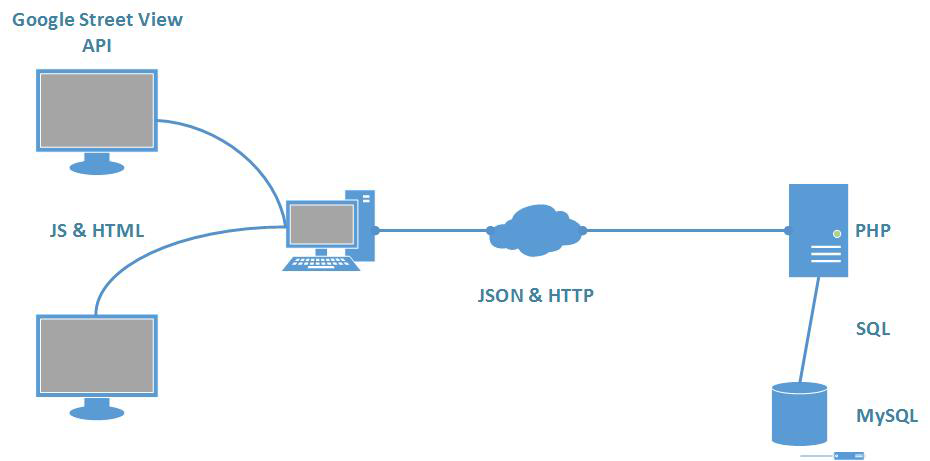
\includegraphics[width=1.0\textwidth]{Architektur.png}
\caption[Architektur der Anwendung]{Architektur der
Anwendung\protect\footnotemark}
\label{fig:Architektur}
\end{figure}
\footnotetext{Quelle: Eigene Darstellung}


In diesem Architekturentwurf ist die Verwendung von vier Technologien vermerkt. Diese sind:
\begin{itemize}
  \item HTML
  \item Javascript
  \item PHP
  \item SQL
\end{itemize}

Diese Technologien sind grundlegend für das Verständnis der entwickelten Software.
Aus diesem Grund werden die wichtigsten Grundlagen zu jeder Technologie nachfolgend erläutert.
Der Fokus liegt dabei immer auf den Teilbereichen, die im vorliegenden Projekt eingesetzt werden.